\documentclass[11pt,a4paper]{article}

\usepackage[utf8]{inputenc}
\usepackage[T1]{fontenc}
\usepackage[margin=1in]{geometry}
\usepackage{amsmath,amssymb,amsthm}
\usepackage{mathtools}
\usepackage{newtxtext,newtxmath}
\usepackage{graphicx}
\usepackage{hyperref}
\usepackage[authoryear,round]{natbib}
\usepackage{enumitem}
\usepackage{booktabs}
\usepackage{xcolor}
\usepackage{caption}
\usepackage{appendix}
\usepackage{microtype}

\graphicspath{{figures/}}
\captionsetup{font=small,labelfont=bf}
\setlist[itemize]{leftmargin=1.25em,itemsep=0.15em,topsep=0.25em}
\setlength{\parindent}{1.05em}
\setlength{\parskip}{0.22em}
\setlength{\abovedisplayskip}{7pt plus 2pt minus 2pt}
\setlength{\belowdisplayskip}{7pt plus 2pt minus 2pt}
\setlength{\textfloatsep}{11pt plus 2pt minus 2pt}
\setlength{\floatsep}{10pt plus 2pt minus 2pt}
\setlength{\intextsep}{10pt plus 2pt minus 2pt}
\renewcommand{\topfraction}{0.9}
\renewcommand{\textfraction}{0.08}
\renewcommand{\floatpagefraction}{0.8}

\definecolor{cBlue}{RGB}{40,80,160}
\definecolor{cOrcid}{HTML}{A6CE39}

\newtheorem{theorem}{Theorem}
\newtheorem{proposition}{Proposition}
\newtheorem{lemma}{Lemma}
\newtheorem{corollary}{Corollary}
\theoremstyle{definition}
\newtheorem{definition}{Definition}
\newtheorem{example}{Example}
\theoremstyle{remark}
\newtheorem{remark}{Remark}

\newcommand{\inner}[2]{\left\langle #1, #2 \right\rangle}
\newcommand{\norm}[1]{\left\lVert #1 \right\rVert}
\newcommand{\abs}[1]{\left\lvert #1 \right\rvert}
\newcommand{\Eqref}[1]{Eq.~\eqref{#1}}

\hypersetup{colorlinks=true, linkcolor=cBlue, citecolor=cBlue, urlcolor=cBlue}

\title{\Large\textbf{Geodesic Provenance, Coherence Gaps, and Subring Structure for Photon-Ring Inference}}
\author{
Jonathan R.\ Landers\\[2pt]
\small Independent researcher\\[-1pt]
\small \texttt{jonathan.robert.landers@gmail.com}\\[2pt]
\small \href{https://orcid.org/0000-0003-1872-6179}{\textcolor{cOrcid}{\Large\textbullet}\,\textcolor{cBlue}{ORCID: 0000-0003-1872-6179}}\\[4pt]
\small \textit{Code and interactive figures:}
\small \href{https://jonland82.github.io/bhex-motivated-photon-ring-analysis/}{\textcolor{cBlue}{project page}}
}
\date{}

\begin{document}
\maketitle

\begin{abstract}
Photon-ring inference is a structured inverse problem where the target is a thin, geometrically informative signal embedded in broader plasma emission, blur, and noise. Direct amplitude readouts can fail before the ring is genuinely unrecoverable; the key question is which properties of the signal and nuisance classes govern that transition. This paper gives a geometric answer, working in a Fourier-domain visibility model where nuisance is constrained by geodesic provenance and the ring signal is decomposed into an exponentially weighted tower of winding-order subrings. Provenance restriction alone yields a monotonic improvement statement: narrowing nuisance to ordinary escaping geodesics cannot increase ring-background coherence. The main theorem then shows that when ring-generating and background-generating geodesic families separate in a criticality index by gap $\Delta$, the aggregate ring-background coherence decays exponentially in $\Delta$. A complementary proposition bounds the truncation error of this tower geometrically. Both results are validated on a dedicated synthetic benchmark with five controlled gap levels and four true subrings per image. On hold-out data, the subring bound upper-bounds empirical coherence on every sample, the designed gap and measured coherence are negatively correlated, and subring-structured estimators halve radius error relative to heuristic and monolithic baselines. The core message is that recoverability is governed not by visual legibility but by the geometry of the signal and nuisance classes and the gap between them---a principle that applies broadly to structured estimation problems with geometrically separated model classes.
\end{abstract}

\smallskip
\noindent\textit{Keywords:} structured inverse problems, statistical recoverability, mutual coherence, operator bounds, signal class geometry, photon-ring inference, interferometric imaging, geodesic provenance

\section{Introduction}

Black-hole imaging has moved from theoretical aspiration to observational reality. The Event Horizon Telescope (EHT) resolved horizon-scale structure in M87$^\ast$ and Sagittarius~A$^\ast$, establishing that black-hole images can be constrained interferometrically on scales set by the photon orbit \citep{EHT2019M87,EHT2022SgrA}. The proposed Black Hole Explorer (BHEX) pushes this program toward longer baselines and cleaner access to the thin photon ring, with the explicit goal of measuring ring geometry and related observables more directly \citep{Johnson2024Vision,Lupsasca2024BHEX,Farah2025Spin}. The physical promise is clear: the photon ring is expected to be more universal, and therefore more geometrically informative, than the broader plasma emission in which it is embedded \citep{Johnson2020Universal,Gralla2019Shadow,Lupsasca2024BHEX}.

The statistical problem is subtler. A long-baseline amplitude heuristic can be compelling when the ring is cleanly visible as an oscillatory signature in Fourier space. But the same measurements can also contain structured contamination from broader crescent-like emission, near-critical shells, scattering, and noise. In that regime, there is a consequential distinction between \emph{readability} and \emph{recoverability}. Readability asks whether the ring is directly legible from a simple summary statistic. Recoverability asks whether the ring can still be stably inferred once the nuisance is modeled explicitly. This paper sharpens that distinction into a precise statistical argument: recoverability is controlled by the coherence between signal and nuisance in observation space, a quantity that admits exponential bounds once both classes are given physical structure and that governs stable estimation in the same fundamental way that mutual coherence governs recovery guarantees in sparse signal models.

Posed formally, the problem is a structured inverse problem with two model classes. The first is the ring family, indexed by a compact geometry parameter and refined here into a low-dimensional subring hierarchy. The second is a nuisance family constrained by provenance: admissible nuisance must be generated by ordinary escaping geodesics rather than by arbitrary Fourier perturbations. The central question is then not whether the data ``look like a ring'' in a raw amplitude plot, but whether the coherence between these two classes is small enough for stable separation.

The paper makes three contributions.
\begin{itemize}
\item It unifies a Fourier-domain mismatch framework with geodesic provenance constraints into a single aggregate subring model, replacing a monolithic ring template with a physically motivated exponential hierarchy while preserving the tractability of a low-dimensional estimator.
\item It shows that provenance restriction alone can only reduce, or at worst preserve, ring-background coherence, and proves that if each subring-background operator pair decorrelates exponentially in a criticality gap $\Delta$, then the aggregate coherence of the full subring tower inherits the same gap-controlled decay.
\item It validates the theorem and the truncation bound on a synthetic benchmark designed specifically to instantiate provenance and subring structure, with five controlled gap levels, four true subrings per image, and a multi-component structured nuisance field.
\end{itemize}

\section{Related Work}

\subsection{Photon rings, interferometry, and BHEX}

The astrophysical motivation is well established. Horizon-scale interferometry now directly constrains the near-black-hole emission morphology in M87$^\ast$ and Sagittarius~A$^\ast$ \citep{EHT2019M87,EHT2022SgrA}, while theoretical work has clarified why the photon ring is such an attractive target: it is produced by strongly lensed trajectories that wind around the black hole with geometry far less sensitive to source details than the broader emission field \citep{Johnson2020Universal,Gralla2019Shadow,Gralla2020Lensing}. BHEX is designed around that opportunity, emphasizing long baselines, ring shape measurement, and interferometric observables tied to photon-ring structure \citep{Johnson2024Vision,Lupsasca2024BHEX,Farah2025Spin}. Proposed detection strategies have focused on extracting photon-ring signatures directly from long-baseline autocorrelations and closure quantities \citep{Tiede2022Photon,Chael2018Closure}.

This paper sits slightly upstream of a full astrophysical forecast. It does not attempt realistic ray tracing, GRMHD calibration, or mission-level sensitivity analysis. Instead, it asks what minimal statistical structure is required for the BHEX intuition to become a usable inverse problem: if the nuisance is physically structured rather than arbitrary, and if the signal is a subring hierarchy rather than a monolithic template, which quantities determine whether the ring remains recoverable?

\subsection{Structured estimation, inverse problems, and learned priors}

Inverse-problem methodology has increasingly emphasized structured priors, data-driven regularization, and learned low-dimensional representations \citep{Arridge2019Survey,Adler2018LPD,Ongie2020Survey}. That literature spans fully learned reconstructions, model-based unrolling \citep{Hammernik2018VN}, plug-and-play methods that substitute learned denoisers for explicit priors \citep{Chan2017PnP}, and hybrid approaches in which a forward model remains explicit but the signal class is restricted by training data or representation learning. In black-hole imaging, PRIMO is an especially relevant example: it learns a compact basis from physically motivated simulations and uses that learned representation to stabilize sparse Fourier inversion \citep{Medeiros2023PRIMO,Psaltis2024PRIMOTheory}.

The present paper is deliberately more austere. It does not learn a black-box reconstructor, nor does it use a large simulation library at inference time. Instead, it develops an analytically tractable estimation framework in which the signal class is narrowed by physical hierarchy and the nuisance class is constrained by provenance. This belongs to the estimation-theoretic tradition of structured signal recovery \citep{Candes2006Robust,Donoho2006CS,Candes2008RIP}: rather than fitting a flexible model, it identifies geometric separation between model classes and derives explicit coherence bounds from that separation. The resulting theory is correspondingly interpretable: the key quantities are coherence, separation gap, and truncation error rather than training loss or network architecture.

\section{Observation Model and Baseline Statistical Picture}

Let $\mathcal H$ be the complex Hilbert space of discretized visibilities. The baseline observation model is
\begin{equation}
y = \alpha g_\theta + q + \varepsilon,
\label{eq:baseline-model}
\end{equation}
where $g_\theta \in \mathcal H$ is a ring template indexed by geometry parameter $\theta$, $\alpha$ is its amplitude, $q$ is structured nuisance, and $\varepsilon$ is noise.

The simplest ring-oriented heuristic estimates amplitude by matched filtering:
\begin{equation}
\hat\alpha_{\mathrm{heur}}
=
\frac{\inner{y}{g_\theta}}{\norm{g_\theta}^2}.
\label{eq:heuristic}
\end{equation}
If nuisance lies in a structured subspace $\mathcal P \subset \mathcal H$, a projection-based structured alternative is
\begin{equation}
\hat\alpha_{\mathrm{model}}
=
\frac{\inner{(I-\Pi_{\mathcal P})y}{(I-\Pi_{\mathcal P})g_\theta}}
{\norm{(I-\Pi_{\mathcal P})g_\theta}^2},
\label{eq:model-est}
\end{equation}
where $\Pi_{\mathcal P}$ denotes orthogonal projection onto $\mathcal P$.

A direct calculation establishes a mismatch bound between the two estimators. With
\[
\mu(g_\theta,\mathcal P):=\frac{\norm{\Pi_{\mathcal P}g_\theta}}{\norm{g_\theta}},
\]
one obtains
\begin{equation}
\abs{\hat\alpha_{\mathrm{heur}}-\hat\alpha_{\mathrm{model}}}
\le
\mu(g_\theta,\mathcal P)\frac{\norm{q}}{\norm{g_\theta}}
+
 \frac{\norm{\varepsilon}}{\norm{g_\theta}}
+
 \frac{\norm{(I-\Pi_{\mathcal P})\varepsilon}}{\norm{(I-\Pi_{\mathcal P})g_\theta}}.
\label{eq:mismatch}
\end{equation}
Equation \eqref{eq:mismatch} makes the paper's governing intuition explicit: the heuristic does not fail merely because nuisance exists, but because nuisance overlaps the ring family. If that overlap is small, the structured and heuristic estimates remain close. If it is large, the heuristic can become biased even before the structured estimator is unstable. The role of mutual coherence as the fundamental obstruction to stable separation has deep roots in sparse recovery theory \citep{Candes2006Robust,Donoho2006CS}; the contribution here is to give it a physical interpretation through geodesic provenance.

A second, more conceptual point concerns identifiability. Suppose a structured estimator fits the full model class,
\begin{equation}
(\hat\alpha,\hat\theta,\hat q)
\in
\arg\min_{\alpha,\theta,q\in\mathcal Q}
\norm{y-\alpha g_\theta-q}_{\mathcal H}^2 + \lambda \mathcal R(q),
\label{eq:structured-fit}
\end{equation}
and assume a local identifiability inequality of the form
\begin{equation}
\norm{\alpha g_\theta + q - \alpha' g_{\theta'} - q'}_{\mathcal H}
\ge
c \bigl(\abs{\alpha-\alpha'} + d(\theta,\theta') + \norm{q-q'}_{\mathcal H}\bigr)
\label{eq:identifiability}
\end{equation}
for nearby triples. Then there is a nonempty regime in which direct peak-reading from amplitude space becomes unreliable while the structured estimator remains stable. In short: the amplitude-readout limit can arrive before the separation limit. That distinction is the baseline narrative which the remainder of the paper sharpens.

\section{Provenance and Subring Refinement}
\label{sec:provenance}

\subsection{Geodesic provenance}

To add physical structure to the nuisance class, let $z=(p,\xi)$ denote a photon initial condition, with associated null geodesic $\gamma_z$. Split initial-condition space into an escape set $E$ and a capture set $C$, where only $E$ contributes to observed data. The key provenance refinement is a further decomposition
\[
E = E_{\mathrm{ring}} \,\dot\cup\, E_{\mathrm{bg}},
\]
where $E_{\mathrm{ring}}$ contains near-critical escaping trajectories that generate the photon ring, while $E_{\mathrm{bg}}$ contains the remaining escaping geodesics. If $T_{E_{\mathrm{ring}}}$ and $T_{E_{\mathrm{bg}}}$ denote the corresponding transport operators to image space and $\mathcal F$ denotes the image-to-visibility map, then
\[
g_\theta = A_r f_\theta,
\qquad
q = A_b h,
\qquad
A_r := \mathcal F T_{E_{\mathrm{ring}}},
\quad
A_b := \mathcal F T_{E_{\mathrm{bg}}}.
\]
This does not change the formal algebra of \eqref{eq:baseline-model}; it changes which nuisance terms are physically admissible.

\subsection{Subring-resolved signal model}

The signal side admits a parallel refinement. The observed photon ring decomposes into a discrete hierarchy of winding-order subrings, with each additional orbit contributing an exponentially dimmer image due to the Lyapunov exponent of the photon orbit \citep{Gralla2020Lensing,Gralla2020Ring}. Let $E_{\mathrm{ring}}=\bigsqcup_{n\ge1} E_n$, where $E_n$ is the $n$th winding class. Define the corresponding visibility templates
\[
g_{\theta,n}=A_{r,n} f_\theta,
\]
with $A_{r,n}$ the transport operator for the $n$th subring family. The aggregate ring template is then
\begin{equation}
g_{\theta}^{(\gamma,N)}
:=
\sum_{n=1}^{N} e^{-\gamma (n-1)} g_{\theta,n},
\qquad \gamma>0,
\label{eq:aggregate-template}
\end{equation}
and the observation model becomes
\begin{equation}
y = \alpha_1 g_{\theta}^{(\gamma,N)} + q + \varepsilon.
\label{eq:aggregate-model}
\end{equation}
This is still a low-dimensional template model. The point of the refinement is not to complicate the estimator, but to avoid treating the signal as a single opaque object when the nuisance has already been given physical structure.

\subsection{Aggregate coherence}

For a nuisance family $Q \subset \mathcal H \setminus \{0\}$ define
\begin{equation}
\mu(g,Q)
:=
\sup_{q\in Q}
\frac{\abs{\inner{g}{q}}}{\norm{g}\,\norm{q}}.
\label{eq:family-coherence}
\end{equation}
Applying the triangle inequality directly to \eqref{eq:aggregate-template} gives the weighted aggregate bound
\begin{equation}
\mu\!\left(g_{\theta}^{(\gamma,N)},Q\right)
\le
\frac{\sum_{n=1}^{N} e^{-\gamma(n-1)} \norm{g_{\theta,n}} \mu(g_{\theta,n},Q)}
{\norm{g_{\theta}^{(\gamma,N)}}}.
\label{eq:weighted-bound}
\end{equation}
Equation \eqref{eq:weighted-bound} is purely algebraic, but it is already useful. It says that the overlap of the full ring tower with nuisance is controlled by subring-wise overlaps, weighted by the same exponential law that defines the signal.

\begin{proposition}[Monotonicity under provenance restriction]
\label{prop:prov-monotone}
Let $Q_{\mathrm{prov}}\subseteq Q\subset \mathcal H \setminus \{0\}$ be nuisance families and let $g\in\mathcal H$ be nonzero. Then
\begin{equation}
\mu(g,Q_{\mathrm{prov}})
\le
\mu(g,Q).
\label{eq:prov-monotone}
\end{equation}
\end{proposition}

\begin{proof}
The claim is immediate from \eqref{eq:family-coherence}: the supremum defining $\mu(g,Q)$ is taken over a larger admissible set than the supremum defining $\mu(g,Q_{\mathrm{prov}})$.
\end{proof}

Proposition~\ref{prop:prov-monotone} is the first payoff of provenance. Before any quantitative separation assumption is imposed, narrowing nuisance to physically admissible escaping backgrounds can only improve, or at worst preserve, the coherence term that enters the mismatch bound \eqref{eq:mismatch}. The same monotonicity holds in the projection picture underlying \eqref{eq:mismatch}: if $\mathcal P_{\mathrm{prov}}\subseteq\mathcal P$ are closed nuisance subspaces, then $\norm{\Pi_{\mathcal P_{\mathrm{prov}}}g}\le \norm{\Pi_{\mathcal P}g}$. Provenance therefore helps twice: it narrows the admissible nuisance family before any geometric gap is imposed, and it creates the setting in which a stronger gap-dependent decay estimate can be asked for.

\section{Gap-Controlled Coherence for Subring Towers}
\label{sec:gap}

The preceding setup becomes genuinely geometric once provenance separation is encoded by a criticality index. Let $\Delta \ge 0$ measure the separation between ring-generating and background-generating trajectories. Proposition~\ref{prop:prov-monotone} says that provenance helps even before a quantitative separation law is available; the next step is to ask when that improvement is not merely monotone but explicitly exponential. The natural operator-level object is the cross operator $A_{b,\Delta}^{*}A_{r,n}$, which measures how strongly the $n$th subring family leaks into the gap-$\Delta$ background family after transport to visibility space. The theorem below shows that exponential decay of these cross operators forces the same decay for the aggregate coherence.

\begin{theorem}[Gap-controlled coherence for aggregate subring templates]
\label{thm:gap-bound}
Fix $N\ge1$ and let
\[
Q_\Delta := \{A_{b,\Delta}h : h\in\mathcal A,\ A_{b,\Delta}h\neq0\}
\]
be a provenance-constrained nuisance family, where $A_{b,\Delta}$ denotes the background transport operator at gap level $\Delta$. Assume:
\begin{enumerate}[label=(\roman*),leftmargin=1.6em,itemsep=0.15em,topsep=0.2em]
\item there exist $\sigma_r,\sigma_b>0$ such that
\[
\norm{A_{r,n}f}\ge \sigma_r \norm{f},
\qquad
\norm{A_{b,\Delta}h}\ge \sigma_b \norm{h}
\]
for all admissible $f$ and $h$;
\item for each subring index $n\in\{1,\dots,N\}$ there exist $c_n>0$ and $\beta>0$ such that
\[
\norm{A_{b,\Delta}^{*}A_{r,n}} \le c_n e^{-\beta\Delta}.
\]
\end{enumerate}
Then
\begin{equation}
\mu\!\left(g_{\theta}^{(\gamma,N)},Q_\Delta\right)
\le
\frac{e^{-\beta\Delta}}{\sigma_r\sigma_b}
\cdot
\frac{\sum_{n=1}^{N} e^{-\gamma(n-1)} c_n \norm{g_{\theta,n}}}
{\norm{g_{\theta}^{(\gamma,N)}}}.
\label{eq:main-bound}
\end{equation}
\end{theorem}

\begin{proof}
Fix $q=A_{b,\Delta}h\in Q_\Delta$. For one subring,
\[
\begin{aligned}
\abs{\inner{g_{\theta,n}}{q}}
&=
\abs{\inner{A_{r,n}f_\theta}{A_{b,\Delta}h}} \\
&=
\abs{\inner{A_{b,\Delta}^{*}A_{r,n}f_\theta}{h}} \\
&\le
\norm{A_{b,\Delta}^{*}A_{r,n}} \norm{f_\theta}\norm{h}.
\end{aligned}
\]
Using the lower bounds $\norm{g_{\theta,n}}=\norm{A_{r,n}f_\theta}\ge \sigma_r \norm{f_\theta}$ and $\norm{q}=\norm{A_{b,\Delta}h}\ge \sigma_b \norm{h}$ yields
\[
\abs{\inner{g_{\theta,n}}{q}}
\le
\frac{c_n e^{-\beta\Delta}}{\sigma_r\sigma_b}
\norm{g_{\theta,n}}\norm{q}.
\]
Summing the weighted subrings,
\[
\begin{aligned}
\abs{\inner{g_{\theta}^{(\gamma,N)}}{q}}
&=
\left|
\sum_{n=1}^{N} e^{-\gamma(n-1)} \inner{g_{\theta,n}}{q}
\right| \\
&\le
\frac{e^{-\beta\Delta}}{\sigma_r\sigma_b}
\norm{q}
\sum_{n=1}^{N} e^{-\gamma(n-1)} c_n \norm{g_{\theta,n}}.
\end{aligned}
\]
Divide by $\norm{g_{\theta}^{(\gamma,N)}}\norm{q}$ and take the supremum over $q\in Q_\Delta$.
\end{proof}

\begin{remark}
Theorem~\ref{thm:gap-bound} has a simple operator-level interpretation. For one subring and one nuisance realization $q=A_{b,\Delta}h$, assumption (i) implies
\[
\frac{\abs{\inner{g_{\theta,n}}{q}}}{\norm{g_{\theta,n}}\norm{q}}
\le
\frac{\norm{A_{b,\Delta}^{*}A_{r,n}}}{\sigma_r\sigma_b}.
\]
Thus assumption (ii) is precisely a decorrelation hypothesis on the cross operator $A_{b,\Delta}^{*}A_{r,n}$. If $A_{r,n}$ and $A_{b,\Delta}$ admit visibility kernels, one standard route to such a hypothesis is the Hilbert--Schmidt estimate
\[
\norm{A_{b,\Delta}^{*}A_{r,n}}
\le
\left(
\int_{E_n}\!\int_{E_{\mathrm{bg}}}
\abs{G_{n,\Delta}(z,z')}^2\,d\nu(z)\,d\nu(z')
\right)^{1/2},
\]
where $G_{n,\Delta}$ is the corresponding gap-dependent cross-Gram kernel. Equation \eqref{eq:main-bound} is therefore the paper's main bridge from phase-space geometry to statistical recoverability: once nuisance is provenance-constrained, the mismatch term in \eqref{eq:mismatch} no longer depends on an abstract overlap parameter. Instead, it decays with the gap between ring-generating and background-generating families, modulated by subring weights and subring norms.
\end{remark}

\begin{corollary}[Mismatch bound for the aggregate subring template]
\label{cor:aggregate-mismatch}
Under the assumptions of Theorem~\ref{thm:gap-bound}, substituting the bound \eqref{eq:main-bound} into the coherence term of \eqref{eq:mismatch} with $g = g_{\theta}^{(\gamma,N)}$ and $q \in Q_\Delta$ gives
\begin{equation}
\abs{\hat\alpha_{\mathrm{heur}} - \hat\alpha_{\mathrm{model}}}
\le
\frac{e^{-\beta\Delta}}{\sigma_r\sigma_b}
\cdot
\frac{\sum_{n=1}^{N} e^{-\gamma(n-1)} c_n \norm{g_{\theta,n}}}
{\norm{g_{\theta}^{(\gamma,N)}}}
\cdot
\frac{\norm{q}}{\norm{g_{\theta}^{(\gamma,N)}}}
+
\text{noise terms}.
\label{eq:aggregate-mismatch}
\end{equation}
The readability/recoverability distinction established in \eqref{eq:mismatch} for a monolithic template therefore carries over to the subring-resolved model unchanged in form: the heuristic-versus-structured gap inherits the exponential decay in $\Delta$. Widening the criticality gap simultaneously makes the ring more recoverable and reduces the bias of the direct amplitude readout.
\end{corollary}

\section{Finite Truncation of the Subring Tower}

The infinite tower suggested by \eqref{eq:aggregate-template} is only useful if it is finitely approximable. The following proposition formalizes that approximation.

\begin{proposition}[Finite-order truncation]
\label{prop:truncation}
Let
\[
g_{\theta}^{(\gamma,\infty)}
:=
\sum_{n=1}^{\infty} e^{-\gamma(n-1)} g_{\theta,n},
\]
and suppose there exists $M_g>0$ such that $\norm{g_{\theta,n}}\le M_g$ for all $n$. Then for every $N\ge1$,
\begin{equation}
\norm{g_{\theta}^{(\gamma,\infty)} - g_{\theta}^{(\gamma,N)}}
\le
\frac{M_g e^{-\gamma N}}{1-e^{-\gamma}}.
\label{eq:tail-bound}
\end{equation}
\end{proposition}

\begin{proof}
By the triangle inequality,
\[
\norm{g_{\theta}^{(\gamma,\infty)} - g_{\theta}^{(\gamma,N)}}
\le
\sum_{n=N+1}^{\infty} e^{-\gamma(n-1)} \norm{g_{\theta,n}}
\le
M_g \sum_{n=N+1}^{\infty} e^{-\gamma(n-1)},
\]
and the remaining series is geometric.
\end{proof}

\section{Synthetic Benchmark}

\subsection{Benchmark design}

Testing the claims of Sections~\ref{sec:provenance} and~\ref{sec:gap} requires data in which the relevant latent structure is directly controllable. Specifically, the benchmark must supply: multiple subrings of known winding order, a variable coherence gap whose effect on ring-background overlap is measurable, a multi-component nuisance field with structured components, and ground-truth coherence values for each sample. These requirements led to a purpose-built synthetic dataset rather than adapting an existing ring-versus-plasma prototype that lacks the necessary internal structure.

\subsection{Data generation}

The dataset contains $120$ tuning images and $60$ hold-out images at $192\times192$ resolution, with random seed $23$. Each sample contains four true subrings. The base ring radius is sampled from $[34,68]$ pixels, the base ring width from $[1.2,2.0]$, the leading amplitude from $[0.55,1.10]$, and the subring decay from $\gamma\in[0.48,1.02]$. The spacing between adjacent subrings is fixed at $1.7$ pixels, while widths grow mildly with winding order.

The nuisance field is deliberately structured. It contains a broad crescent, a near-critical shell, and two diffuse blobs. The designed gap $\Delta$ enters through the shell amplitude by the factor
\[
\exp(-1.15 \Delta),
\]
with gap levels $\{0.45,0.85,1.25,1.65,2.05\}$. This is not a ray-traced criticality index; it is a synthetic control intended to instantiate the gap variable in Theorem~\ref{thm:gap-bound}. Gaussian scattering blur, center jitter, and additive noise are then applied. The resulting images are converted to visibilities by FFT, and each sample stores the true aggregate coherence, the subring-wise coherence terms, and the finite-truncation envelopes implied by \eqref{eq:tail-bound}.

\begin{figure}[!t]
\centering
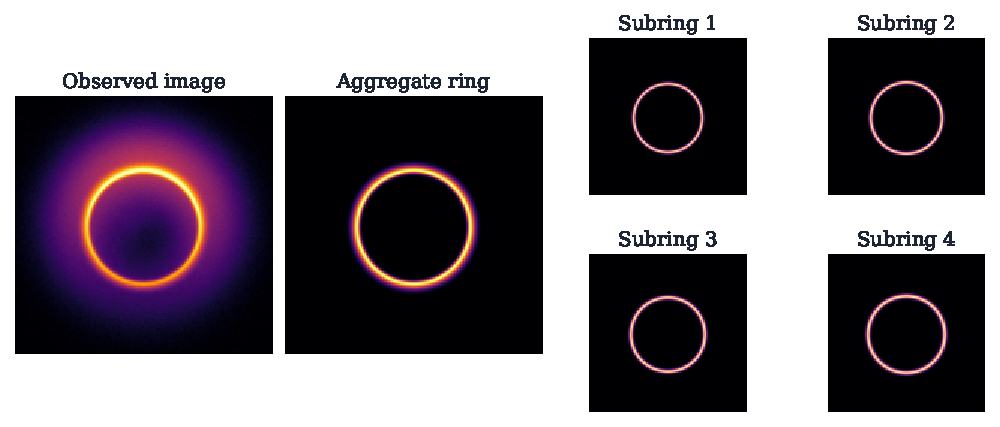
\includegraphics[width=0.93\textwidth]{fig_setup.pdf}
\caption{Representative hold-out sample from the dedicated coherence/subring benchmark. The observed image combines structured nuisance with an aggregate ring, while the signal side is generated from four exponentially weighted subrings.}
\label{fig:setup}
\end{figure}

\subsection{Inference methods}

The goal is radius recovery. Four methods are evaluated: an \textbf{amplitude heuristic} (direct readout from visibility amplitudes, weighted toward larger Fourier radii); a \textbf{monolithic ring model} (the structured estimator \eqref{eq:structured-fit} with a single ring template); a \textbf{two-subring model} (the same estimator with an aggregate template bank over radius and $\gamma$); and a \textbf{four-subring model} (the same estimator with a four-subring template bank). The structured models solve
\begin{equation}
(\hat\alpha,\hat k,\hat q)
\in
\arg\min_{\alpha,k,q}
\norm{y-\alpha g_k-q}_2^2 + \lambda \norm{Hq}_2^2,
\label{eq:benchmark-estimator}
\end{equation}
where $k$ indexes a template bank and $H$ penalizes high-frequency nuisance content. The regularization parameter $\lambda$ is tuned on $36$ randomly selected tuning images over the grid $\{0.5,1.5,4,10\}$. The best values are $4.0$ for the monolithic model and $10.0$ for both subring models.

\subsection{Metrics}

Three quantitative outputs matter most: \textbf{radius MAE} (mean absolute error of the recovered base radius), \textbf{ring relative MSE} (relative mean-squared error of the reconstructed aggregate ring image), and \textbf{gamma MAE} (absolute error in the recovered subring decay parameter, for the subring models). The benchmark additionally tracks the empirical aggregate coherence of each sample, the weighted subring bound from \eqref{eq:weighted-bound}, and the true versus bounded truncation tail fractions.

\section{Results}

\subsection{Global recovery performance}

The main quantitative comparison is shown in Table~\ref{tab:main-results}. The two-subring model achieves the best geometry recovery, with hold-out radius MAE $0.424$ pixels. The four-subring model is nearly as good on geometry at $0.433$ pixels and clearly best on ring reconstruction, with mean relative ring MSE $0.231$. Both subring models outperform the monolithic model by roughly a factor of two in radius MAE and also dominate the direct amplitude heuristic.

\begin{table}[t]
\centering
\small
\begin{tabular}{lcccc}
\toprule
Method & Radius MAE & 90\% CI & Ring rel. MSE & $\gamma$ MAE \\
\midrule
Amplitude heuristic & 0.883 & 0.792--0.956 & -- & -- \\
Monolithic ring model & 0.833 & 0.717--0.959 & 0.564 & -- \\
Two-subring model & 0.424 & 0.360--0.496 & 0.400 & 0.242 \\
Four-subring model & 0.433 & 0.378--0.505 & 0.231 & 0.243 \\
\bottomrule
\end{tabular}
\caption{Hold-out performance on the coherence/subring benchmark. Two subrings are best for geometry recovery; four subrings are best for full ring reconstruction.}
\label{tab:main-results}
\end{table}

Measured against the monolithic structured model, the two-subring model reduces hold-out radius MAE by $49.1\%$, while the four-subring model reduces it by $48.1\%$. Relative to the amplitude heuristic, the reductions are $51.9\%$ and $51.0\%$, respectively. On morphology, the four-subring model reduces mean relative ring MSE by $59.1\%$ relative to the monolithic model, while the two-subring model reduces it by $29.0\%$, making the geometry-versus-morphology tradeoff quantitatively explicit rather than anecdotal. Those improvements are too large to be read as marginal tuning effects; they indicate that the added signal structure is carrying information that a single ring template leaves unused.

\subsection{Representative gap regimes}

Figure~\ref{fig:gap-cases} provides a qualitative cross-section of the benchmark at three designed gap levels. As the nuisance changes from relatively ring-adjacent leakage to broader, more clearly separated contamination, the observed image can become increasingly background-dominated even though the true aggregate ring remains thin and stable. The rightmost column shows that the four-subring model still recovers the correct geometry across this range, which is the qualitative counterpart of the quantitative gap and coherence trends below.

\begin{figure}[t]
\centering
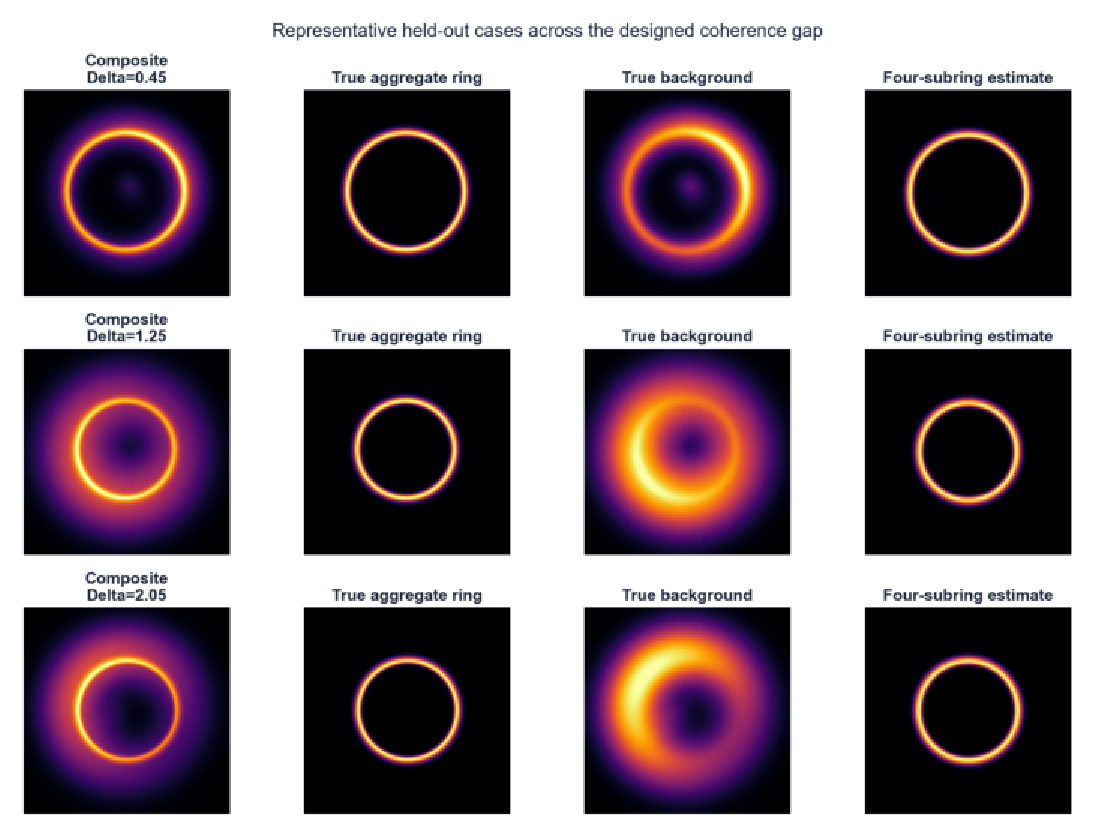
\includegraphics[width=\textwidth]{fig_gap_cases.pdf}
\caption{Representative hold-out cases across low-, mid-, and high-gap regimes. Each row shows the composite observation, the true aggregate ring, the true background, and the four-subring estimate. The designed gap changes how ring-adjacent the nuisance field is, while the subring-structured estimator retains the correct ring geometry across the range.}
\label{fig:gap-cases}
\end{figure}

\subsection{Gap-controlled coherence appears in the data}

Theorem~\ref{thm:gap-bound} predicts that increased separation between ring-generating and background-generating families should reduce aggregate coherence. Figure~\ref{fig:gap-bound} shows that the synthetic benchmark indeed behaves that way. On hold-out data, the designed gap and empirical coherence are negatively correlated ($r=-0.560$), and the median coherence across gap levels is well fit by
\[
\mu_{\mathrm{med}}(\Delta) \approx 0.626 e^{-0.149\Delta}.
\]
The right panel verifies the second half of the theorem's story: the weighted subring bound upper-bounds the empirical aggregate coherence on every hold-out sample, so the coverage fraction is exactly $1.0$ in this experiment.

\begin{figure}[t]
\centering
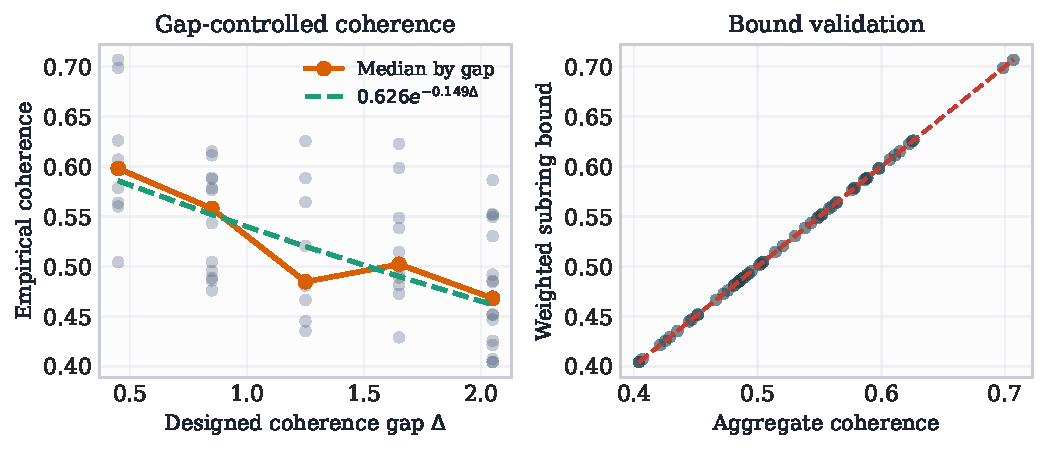
\includegraphics[width=\textwidth]{fig_gap_bound.pdf}
\caption{Left: empirical ring-background coherence decreases as the designed gap widens. Right: the weighted subring bound upper-bounds empirical aggregate coherence on every hold-out sample.}
\label{fig:gap-bound}
\end{figure}

\subsection{Performance degrades with coherence, but not equally}

Figure~\ref{fig:error-coherence} shows a second empirical pattern: all methods become worse as empirical coherence rises, but they do not deteriorate at the same rate. The monolithic model tracks the amplitude heuristic fairly closely, while the two- and four-subring models remain substantially lower across the whole coherence range.

\begin{figure}[t]
\centering
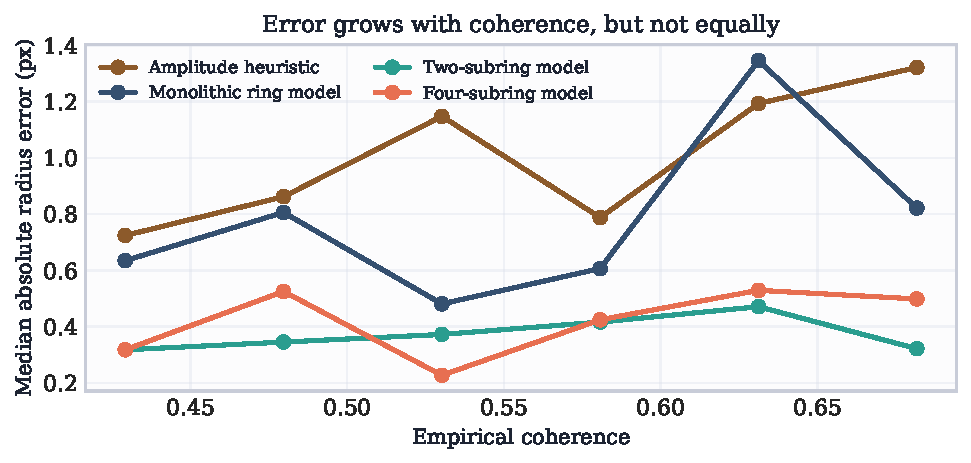
\includegraphics[width=\textwidth]{fig_error_coherence.pdf}
\caption{Median radius error as a function of empirical coherence. Recovery degrades as nuisance overlap rises, but the subring models degrade more slowly than the heuristic or monolithic baseline.}
\label{fig:error-coherence}
\end{figure}

The bucketed numbers make that concrete. In the highest-coherence third of the hold-out set, the monolithic model has mean absolute radius error $1.025$ pixels, versus $0.546$ for the two-subring model and $0.560$ for the four-subring model. Even in the lowest-coherence third, where the task is easiest, the two-subring model remains best.

\begin{table}[t]
\centering
\small
\begin{tabular}{lcccc}
\toprule
Coherence band & Heuristic & 1-subring & 2-subring & 4-subring \\
\midrule
Low coherence & 0.780 & 0.730 & 0.320 & 0.382 \\
Mid coherence & 0.895 & 0.745 & 0.407 & 0.357 \\
High coherence & 0.975 & 1.025 & 0.546 & 0.560 \\
\bottomrule
\end{tabular}
\caption{Mean absolute radius error by empirical-coherence tercile on the hold-out set. Subring models retain a substantial advantage even when ring-background overlap is strongest.}
\label{tab:bucket-results}
\end{table}

\subsection{Only a few subrings carry most of the recoverable signal}

Proposition~\ref{prop:truncation} predicts exponentially controlled tail error. Figure~\ref{fig:methods-truncation} shows that the synthetic data are consistent with that picture. If only the leading subring is retained, the omitted tail carries about $0.507$ of the total ring norm on average. Retaining the first two subrings cuts that to $0.238$, and retaining the first three cuts it to $0.086$. The geometric envelope from \eqref{eq:tail-bound} is conservative but correctly ordered, with mean values $0.721$, $0.361$, and $0.184$.

This explains a central empirical fact in Table~\ref{tab:main-results}: the two-subring model already captures most of the geometry. The four-subring model reconstructs the full aggregate ring more faithfully, but the marginal benefit for radius recovery is small because the omitted tail is already modest after the first two components.

\begin{figure}[t]
\centering
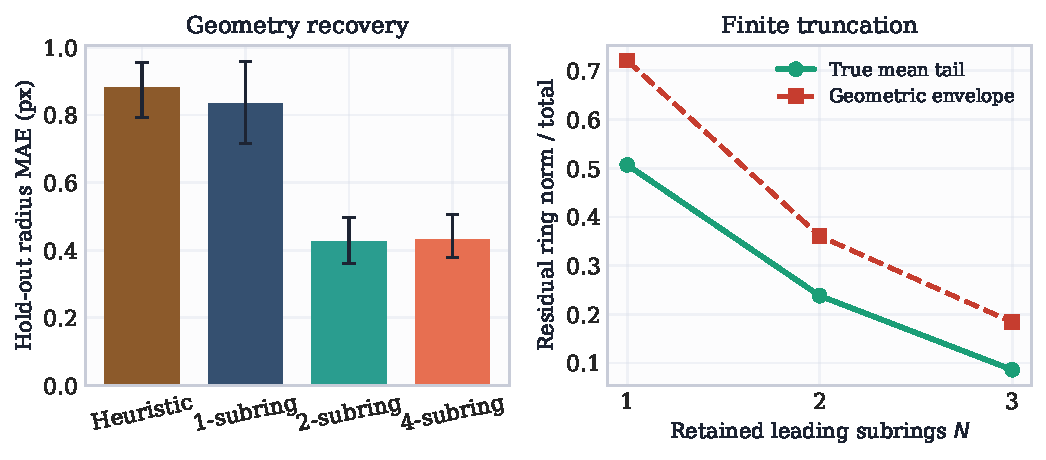
\includegraphics[width=\textwidth]{fig_methods_truncation.pdf}
\caption{Left: global method comparison in hold-out radius MAE. Right: true truncation tail fraction and the geometric envelope from Proposition~\ref{prop:truncation}. A few leading subrings carry most of the recoverable signal.}
\label{fig:methods-truncation}
\end{figure}

\section{Discussion}

The scope of this paper is deliberately focused, and the limitations are worth naming. The coherence gap $\Delta$ is a synthetic control variable: it is designed to instantiate the phase-space separation assumed in Theorem~\ref{thm:gap-bound}, not to replace a ray-traced criticality index. The benchmark components---crescent, shell, blobs---are simple analytical shapes rather than GRMHD emission fields. And the statistical model is low-dimensional by design, intended to isolate a specific structural claim rather than to serve as a general-purpose reconstruction pipeline.

Those constraints are also inseparable from the paper's argument. The central question is not whether one can produce a realistic synthetic black-hole observation, but whether a small amount of physically motivated structure already changes the inverse problem qualitatively. The answer is yes. A provenance-constrained nuisance class converts an abstract overlap parameter into a geometrically decaying quantity; a subring-resolved signal class captures structure that a monolithic template discards; and together they extend the range over which stable recovery is possible even after direct amplitude readouts lose reliability.

The claims of this paper are about model class geometry, not about a specific instrument or computational architecture. The structured inverse-problem literature has demonstrated repeatedly that restricting the signal class to a well-chosen low-dimensional family can stabilize reconstructions that are otherwise ill-posed \citep{Candes2006Robust,Donoho2006CS,Candes2008RIP,Arridge2019Survey,Adler2018LPD,Ongie2020Survey}. Methods such as PRIMO operationalize this principle for astrophysical imaging through learned compact bases \citep{Medeiros2023PRIMO,Psaltis2024PRIMOTheory}. The present contribution is complementary and more minimal: it shows that even a purely analytical restriction---geodesic provenance on the nuisance side, subring hierarchy on the signal side---yields a mathematically transparent and empirically meaningful gain, one that can be traced to a single quantity, $\mu(g_\theta^{(\gamma,N)}, Q_\Delta)$, rather than to training loss or network architecture. That this gain arises from geometric separation between model classes, and not from any domain-specific property of black-hole imaging, suggests the framework carries over to other structured estimation problems where signal and nuisance can be assigned to physically or statistically distinct generating families.

\section{Conclusion}

The photon ring is attractive as an inference target precisely because its geometry is less sensitive to astrophysical details than the broader emission field surrounding it. But that geometric advantage is only useful if the ring can be separated from the nuisance reliably, and amplitude-space readability is an unreliable proxy for that separability. This paper has shown that the relevant quantity is coherence: the normalized inner product between ring and nuisance families in visibility space. When nuisance is constrained by geodesic provenance and the signal is resolved into a winding-order subring hierarchy, coherence admits a gap-controlled exponential bound, the infinite tower is finitely approximable, and both facts translate into measurable recovery gains on a controlled synthetic benchmark.

The broader lesson is geometric. In inverse problems of this kind, what determines stable recovery is not whether the target signal is visually conspicuous, but whether the signal class and nuisance class remain sufficiently separated in the observation space. Geodesic provenance and subring structure each narrow one side of that gap, and narrowing either side makes the whole problem easier. That principle is simple, but it has concrete and quantifiable consequences for photon-ring inference.

\bibliographystyle{plainnat}
\bibliography{coherence_gaps_subrings}

\end{document}
